\documentclass[a4paper,10.5pt]{article}

\usepackage[utf8]{inputenc}
\usepackage[T1]{fontenc}
\usepackage{fancyhdr} % pour personnaliser les en-têtes
\usepackage{lastpage}
\usepackage[frenchb]{babel}
\usepackage{amsfonts,amssymb}
\usepackage{amsmath,amsthm}
\usepackage{paralist}
\usepackage{enumerate}
\usepackage{xspace}
\usepackage{xcolor}
\usepackage{variations}
\usepackage{xypic}
\usepackage{eurosym,multicol}
\usepackage{graphicx}
\usepackage[np]{numprint}
\usepackage{hyperref} 
\usepackage{setspace}
\usepackage{listings} % pour écrire des codes avec coloration syntaxique  

\usepackage{tikz}
\usetikzlibrary{calc, arrows, plotmarks,decorations.pathreplacing}
\usepackage{colortbl}
\usepackage{multirow}
\usepackage[top=1.5cm,bottom=1.5cm,right=1.5cm,left=1.5cm]{geometry}

\newtheorem{defi}{Définition}
\newtheorem{thm}{Théorème}
\newtheorem{thm-def}{Théorème/Définition}
\newtheorem{rmq}{Remarque}
\newtheorem{prop}{Propriété}
\newtheorem{cor}{Corollaire}
\newtheorem{lem}{Lemme}
\newtheorem{ex}{Exemple}
\newtheorem{cex}{Contre-exemple}
\newtheorem{prop-def}{Propriété-définition}
\newtheorem{exer}{Exercice}
\newtheorem{nota}{Notation}
\newtheorem{ax}{Axiome}
\newtheorem{appl}{Application}
\newtheorem{csq}{Conséquence}
%\def\di{\displaystyle}


\newcommand{\vtab}{\rule[-0.4em]{0pt}{1.2em}}
\newcommand{\V}{\overrightarrow}
\renewcommand{\thesection}{\Roman{section} }
\renewcommand{\thesubsection}{\arabic{subsection} }
\renewcommand{\thesubsubsection}{\alph{subsubsection} }
\newcommand{\C}{\mathbb{C}}
\newcommand{\R}{\mathbb{R}}
\newcommand{\Q}{\mathbb{Q}}
\newcommand{\Z}{\mathbb{Z}}
\newcommand{\N}{\mathbb{N}}


\definecolor{vert}{RGB}{11,160,78}
\definecolor{rouge}{RGB}{255,120,120}
% Set the beginning of a LaTeX document
\pagestyle{fancy}
\lhead{}\chead{}\rhead{}\lfoot{Chapitre 5 - Cours}\cfoot{\thepage/..}\rfoot{M. Botcazou}\renewcommand{\headrulewidth}{0pt}\renewcommand{\footrulewidth}{0.4pt}

\begin{document}
	%\tableofcontents

	$$\fbox{\text{\Large{ Chapitre 5 : Premières notions de fonction}}}$$
	
	%$$\fbox{\text{\Large{ \begin{minipage}{0.9\linewidth } \centering\hfil\\ ......\hfill \\\hfill \\\end{minipage} }}}$$
	



\renewcommand{\arraystretch}{1.5}
$$\begin{tabular}{|l|l|}
\hline
\textbf{Contenus} & \textbf{Capacités attendues} \\
\hline 
$\bullet$  Fonctions réelles définies sur un intervalle& $\bullet$   Comparer $f(a)$ et $f(b)$ numériquement ou graphiquement.\\
 ou une réunion d'intervalles réels. & $\bullet$  Résoudre graphiquement ou algébriquement une équation\\
$\bullet$  Tracer la courbe représentative d'une fonction. &  ou une inéquation du type $f(x)=k$, $f(x)<k$, $f(x)\geq k$.\\
$\bullet$  Croissance, décroissance, monotonie sur un    & $\bullet$ Relier représentation graphique et tableau de variations.\\
intervalle, tableau de variations. & $\bullet$ Déterminer graphiquement les extremums d’une fonction \\
$\bullet$  Signe d'une fonction sur un  intervalle, &  sur un intervalle.\\
 tableau de signes. & $\bullet$ Exploiter un logiciel de géométrie dynamique \\
$\bullet$  Maximum, minimum d’une fonction sur & $\bullet$   Modéliser un problème à l'aide des fonctions. \\
un intervalle. &\\
\hline
\end{tabular}$$
\hfill\\[-0.2cm]
\setstretch{1,5}
\noindent\textbf{Démonstrations :}
\begin{enumerate}[$\square$]
	\item Étudier la position relative des courbes d’équation $y=x$ , $y= x^2$ et $ y=x^3$ pour $x\geq 0$.
\end{enumerate}

\section{Vocabulaire et applications:}
\subsection{Le vocabulaire:}
\subsubsection{Notion de fonction réelle:}
\medskip

\noindent\fcolorbox{vert}{white}{\begin{minipage}{1\linewidth}\begin{defi}\hfill\\
Une fonction réelle $f$ définie sur un intervalle $I$ est un objet mathématiques qui à tout $x\in I$ lui associe un \dots\dots \dots \quad \  % \textbf{unique} 
nombre réel noté  \dots\dots \\%$f(x)$. 
\end{defi}
\end{minipage}\hfill\\}\hfill\\
\begin{rmq}
Le nombre $f(x)$ est obtenu grâce à une transformation de la variable $x$.
\end{rmq}
\begin{exer}
Transformer les protocoles de calculs suivants à l'aide d'une écriture fonctionnelle:
 \begin{enumerate}
\item \textbf{Exemple:} Pour tout $x$ dans l'intervalle $[0;4]$ la fonction $f$ le multiplie par $3$ et lui soustrait $5$: 
\item[$\bullet$]$\text{Pour tout } x\in[0;4] , f(x)= 3x-5. $
\item Pour tout $x$ dans l'intervalle $[2;7]$ la fonction $g$ le multiplie par $1$ et lui ajoute $2$: 
\item[$\bullet$].\dotfill 
\item Pour tout $x$ dans l'intervalle $]-3;-1]$ la fonction $h$ le multiplie par $0$ et lui ajoute $12$: 
\item[$\bullet$].\dotfill 
\item Pour tout $x$ dans l'intervalle $]0;+\infty[$ la fonction $k$ le met au carré et lui ajoute $-1$: 
\item[$\bullet$].\dotfill 
\item Pour tout $x$ dans l'intervalle $ ]-\infty;+\infty[  \ =   \R$ la fonction $m$ le duplique en deux, elle met le premier au cube, puis elle met le second au carré, enfin elle ajouter les deux ensemble:  
\item[$\bullet$].\dotfill 
\item Pour tout $x$ dans l'intervalle $ [0;+\infty[  \ =   \R^+$ la fonction $n$ lui ajoute $1$ et prend la racine carrée de cette somme.   
\item[$\bullet$].\dotfill 
 \end{enumerate}
\end{exer} 
\newpage
\subsubsection{Notion de l'image d'un nombre par une fonction:}
\noindent\fcolorbox{vert}{white}{\begin{minipage}{1\linewidth}\begin{defi}\hfill\\
Soit $f$ une fonction définie sur un intervalle $I$.\\ Pour tout $a\in I$ on note $f(a)$ \  \dots\dots\dots \dots\dots\dots \dots\dots\dots \dots\dots\dots \dots\dots\dots \dots\dots\dots  \\% l'image de $a$ par la fonction $f$
\end{defi}
\end{minipage}\hfill\\}\hfill\\

\begin{ex}\hfil\\[-0.6cm]
\begin{enumerate}
\item Si pour tout  $x\in\R , f(x)= 3x-5 $. Alors l'image de $4$ par la fonction $f$ est:  $f(4)= \dots\dots \dots\dots\dots \dots$
\item Si pour tout  $x\in\R , f(x)= x^2-1 $. Alors l'image de $2$ par la fonction $f$ est:  $\dots\dots$   $= \dots\dots \dots\dots\dots \dots$
\item Si pour tout  $x\in\R , f(x)= x^3 $. Alors l'image de $-1$ par la fonction $f$ est:  $\dots\dots$   $= \dots\dots \dots\dots\dots \dots$
\item Si pour tout  $x\in\R^+ , f(x)= \sqrt{x} $. Alors l'image de $49$ par la fonction $f$ est:  $\dots\dots$   $= \dots\dots \dots\dots\dots \dots$
\end{enumerate}
\end{ex}
\subsubsection{Notion d'antécédent d'un nombre par une fonction:}

\noindent\fcolorbox{vert}{white}{\begin{minipage}{1\linewidth}\begin{defi}\hfill\\
Soit $f$ une fonction définie sur un intervalle $I$.\\ Pour tout $y\in \R$ nous dirons que $y$ admet un antécédent par la fonction $f$ \textbf{si il existe} \dots\dots\dots \dots\dots\\ % $x\in I$ 
 tel que:  \dots\dots\dots\dots\dots\dots\dots\dots\\ % $f(x) = y
\end{defi}
\end{minipage}\hfill\\}\hfill\\
\begin{ex}\hfil\\[-0.6cm]
\begin{enumerate}
\item Si pour tout  $x\in\R , f(x)= x+5 $. Alors le nombre  $10$ admet un antécédent par la fonction $f$ car:\\
.\dotfill\\
.\dotfill
\item Si pour tout  $x\in\R , f(x)= x-3 $. Alors le nombre  $-3$ admet un antécédent par la fonction $f$ car:\\
.\dotfill\\
.\dotfill

\item Si pour tout  $x\in\R , f(x)= 2x $. Alors le nombre  $8$ admet un antécédent par la fonction $f$ car:\\
.\dotfill\\
.\dotfill

\item Si pour tout  $x\in\R , f(x)= 5x +1$. Alors le nombre  $6$ admet un antécédent par la fonction $f$ car:\\
.\dotfill\\
.\dotfill

\item Si pour tout  $x\in\R , f(x)= 7x +9$. Alors le nombre  $12$ admet un antécédent par la fonction $f$ car:\\
.\dotfill\\
.\dotfill
\end{enumerate}
\end{ex}

\begin{rmq}
Lorsque nous cherchons l'antécédent de $y\in\R$ par la fonction $f$ il faudra résoudre l'équation: 

\centering \large$ f(x)=y$ 
\flushleft \normalsize
\end{rmq}\hfill\\[-2.5cm]
\begin{rmq}\hfill\\[-0.7cm]

\begin{enumerate}[$\bullet$]
\item Pour certains nombres réels $y\in\R$, il \textbf{n'existe pas d'antécédent} de $y$  par une fonction $f$ donnée. 
\item Pour certains nombres réels $y\in\R$, \textbf{il existe plusieurs antécédents} de $y$ par une fonction $f$ donnée. 
\end{enumerate}
\end{rmq}

\begin{ex}\hfil\\[-0.6cm]
	\begin{enumerate}
		\item Si pour tout  $x\in\R , \ f(x)= x^2 $. 
		\begin{enumerate}[$\square$]
			\item Le nombre  $-5$ admet-il un antécédent par la fonction $f$ ?\\
			.\dotfill\\
			.\dotfill 
			\item Donner les antécédents du nombre $25$ par la fonction $f$.\\
			.\dotfill\\
			.\dotfill  
		\end{enumerate}	
	\item Si pour tout  $x\in\R , \ g(x)= x^2 -2 $. 
	\begin{enumerate}[$\square$]
	\item Le nombre  $-3$ admet-il un antécédent par la fonction $g$ ?\\
	.\dotfill\\
	.\dotfill 
	\item Donner les antécédents du nombre $7$ par la fonction $g$.\\
	.\dotfill\\
	.\dotfill\\  
\end{enumerate} 
	\end{enumerate}
\end{ex}
\subsubsection{Exercices d'applications:}
\begin{exer}Pour tout  $x\in\R$ on défini $f(x)= (x-5)(x+5)$ et $g(x)=(x+3)^2$ 
	\begin{enumerate}
		\item Donner l'image de $\dfrac{4}{5}$ par la fonction $f$.\\
		.\dotfill\\
		.\dotfill\\
		.\dotfill 
		\item Donner l'image de $\sqrt{3}$ par la fonction $g$.\\
		.\dotfill\\
		.\dotfill\\
		.\dotfill
		\item Donner les antécédents de $0$ par la fonction $f$.\\
		.\dotfill\\
		.\dotfill\\		
		.\dotfill\\
		.\dotfill
		\item Donner les antécédents de $36$ par la fonction $g$.\\
		.\dotfill\\
		.\dotfill\\		.\dotfill\\
		.\dotfill
	\end{enumerate}

	
\end{exer}

\noindent \textbf{\textcolor{purple}{$
\includegraphics[scale=0.05]{logo-td.png}$ \ Exercice 36 p.95 - Exercice 45 p.96 - Exercice 36 p.95 }}
 
\section{Courbe représentative et lecture graphique:}

\subsection{Courbe représentative d'une fonction:}

\noindent\fcolorbox{vert}{white}{\begin{minipage}{1\linewidth}
		\begin{defi}\hfill\\
			Soient $f$ une fonction définie sur un intervalle $D$ et $(O,I,J)$ un repère du plan. On appelle \  \dots\dots\dots \dots\\\dots\dots \dots\dots\dots \dots\dots\dots %courbe représentative
			de la fonction $f$ sur l'intervalle $D$ l'ensemble des points du plan $\mathcal{C}_f$ tels que:
			$$ \mathcal{C}_f := \left\{\dots\dots\dots \dots\dots\dots \dots\dots\dots \dots\dots\dots \right\}$$ \\%(x;f(x)) tel que x$\inD \hfill
			\\[-1.8cm] 
		\end{defi}
	\end{minipage}\hfill\\}\hfill\\

\begin{rmq}
	Pour tracer la courbe représentative de la fonction $f$ sur l'intervalle $D$ nous allons faire un tableau de valeurs en piochant des valeurs de $x$ dans l'intervalle $D$ et en calculant $f(x)$. Plus il y aura de valeurs plus la courbe sera précise. 
\end{rmq}

\begin{exer}
	On nous donne ci-dessous un tableau de valeurs pour la fonction $f$ définie sur l'intervalle $[-2;2.5]$, les images $f(x)$ on déjà été calculées dans ce tableau. Tracer avec les données de ce tableau deux approximations possibles de $\mathcal{C}_f$.
\begin{center}
\begin{tabular}{|c|l|l|l|l|l|l|l|l|l|l|}
	\hline
	$x \in [-2;2.5]$&-2&-1.5&-1&-0.5&0&0.5&1&1.5&2&2.5 \\
	\hline
	$f(x)$&-2&-2.5&-3&-2.25&-0.5&0.5&2&1.5&2.5&3 \\
	\hline
\end{tabular}

\medskip



$$\begin{tikzpicture}[scale=0.6]
\draw[dotted] (-5,-7) grid (6,7);
\draw [->, line width = 1pt, >=latex'](-5,0) -- (6,0);
\draw [->, line width = 1pt, >=latex'](0,-7) -- (0,7);
\draw (0,2) node{$+$} node[above left]{$J$};
\draw (2,0) node{$+$} node[below left]{$I$};
\draw (0,0) node{$+$} node[below left]{$O$};
\draw (0,6.8) node[below left]{$y$};
\draw (5.8,0) node[below left]{$x$};
\end{tikzpicture}$$
\end{center}	
\end{exer}
\begin{rmq}
	La courbe représentative $\mathcal{C}_f$ d'une fonction $f$ devient précise plus on choisit un nombre important de $x$ sur l'axe des abscisses pour ensuite calculer le nombre $f(x)$ et obtenir un point de $\mathcal{C}_f$. 
\end{rmq}
\begin{exer}
	En vous inspirant de l'exercice 3 qui précède, tracer sur votre cahier d'exercices la courbe représentative de la fonction g sur l'intervalle $[-2;2.5]$ sachant que: 
	
	$$\text{Pour tout } x \in\R, \ g(x)= x^2-x$$
\end{exer}
\newpage
\subsection{Lecture graphique avec la courbe représentative d'une fonction:}
\subsubsection{Lire les images et les antécédents:}
\fcolorbox{blue}{white}{
	\begin{minipage}{0.95\linewidth}
		\hfill\\
		\noindent\textbf{\underline{Trouver l'image d'un nombre $x_0$ par la fonction $f$:}}\\
		\begin{minipage}[t]{0.5\linewidth}
			\begin{enumerate}[I/]
				\item Trouver le nombre $x_0$ sur l'axe des abscisses.
				\item Monter ou bien descendre jusqu'à toucher la courbe $\mathcal{C}_f$.
				\item Se déplacer horizontalement en restant à la même hauteur pour retrouver l'axe des ordonnées.
				\item Lire le nombre associé $f(x_0)$ qui est l'image de $x_0$ par la fonction $f$. 
			\end{enumerate}
			
		\end{minipage}
		\begin{minipage}[t]{0.5\linewidth}
			$$\shorthandoff{:}\begin{tikzpicture}[scale=1]
			\draw[dotted] (-2,-1) grid (2,4);
			\draw [->, line width = 1pt, >=latex'](-2,0) -- (2,0);
			\draw [->, line width = 1pt, >=latex'](0,-1) -- (0,4);
			\draw (0,1) node{$+$} node[above left]{$J$};
			\draw (1,0) node{$+$} node[below left]{$I$};
			\draw (0,0) node{$+$} node[below left]{$O$};
			\draw[domain=-2:2,samples=100,color=blue] plot ({\x},{\x*\x});
			\draw [line width = 1.5pt, color=red, dotted] (-1.5,0) -- (-1.5,1.5*1.5);
			\draw (-1.5,0) node[below]{$x_0$};
			\draw (-1.5,1.5*1.5) node {$\times$};
			\draw [line width = 1.5pt, color=red, dotted] (-1.5,1.5*1.5) -- (0,1.5*1.5);
			\draw (0,1.5*1.5) node[right]{$f(x_0)$};
			\end{tikzpicture}\shorthandon{:}$$
		\end{minipage}	
	\hfill\\	
	\end{minipage}
}
\hfill\\

\fcolorbox{blue}{white}{
	\begin{minipage}{0.95\linewidth}
		\hfill\\
		\noindent\textbf{\underline{Trouver le(s) antécédent(s) de $y_0$ par $f$ si il(s) existe(nt):}}\\
		\begin{minipage}[t]{0.5\linewidth}
			\begin{enumerate}[I/]
				\item Trouver le nombre $y_0$ sur l'axe des ordonnées.
				\item Se déplacer horizontalement en restant à la même hauteur pour trouver si il existe un ou des points de $\mathcal{C}_f$. 
				\item Partir des points de $\mathcal{C}_f$ trouvés puis monter ou bien descendre jusqu'à toucher l'axe des abscisses.
				\item Lire les valeurs $x_0$ et $x_1$ qui sont les antécédents de $y_0$ par la fonction $f$. 
			\end{enumerate}
			
		\end{minipage}
		\begin{minipage}[t]{0.5\linewidth}
			$$\shorthandoff{:}\begin{tikzpicture}[scale=1]
			\draw[dotted] (-2,-1) grid (2,4);
			\draw [->, line width = 1pt, >=latex'](-2,0) -- (2,0);
			\draw [->, line width = 1pt, >=latex'](0,-1) -- (0,4);
			\draw (0,1) node{$+$} node[above left]{$J$};
			\draw (1,0) node{$+$} node[below left]{$I$};
			\draw (0,0) node{$+$} node[below left]{$O$};
			\draw[domain=-2:2,samples=100,color=blue] plot ({\x},{\x*\x});
			\draw [line width = 1.5pt, color=brown, dotted] (-1.5,0) -- (-1.5,1.5*1.5);
			\draw (-1.5,0) node[below]{$x_0$};
			\draw [line width = 1.5pt, color=brown, dotted] (-1.5,1.5*1.5) -- (1.5,1.5*1.5);
			\draw (0,2.25) node[above right]{$y_0$};
			\draw [line width = 1.5pt, color=brown, dotted] (1.5,0) -- (1.5,1.5*1.5);
			\draw (1.5,0) node[below]{$x_1$};
			\draw (-1.5,1.5*1.5) node {$\times$};
			\draw (1.5,1.5*1.5) node {$\times$};
			\end{tikzpicture}\shorthandon{:}$$
		\end{minipage}	
		\hfill\\	
	\end{minipage}}
\hfill\\
\begin{exer}\hfill\\
	\begin{minipage}[t]{1.0\linewidth}
		On considère une fonction G définie sur $\mathbb{R}$ dont on donne une représentation graphique ci-dessous:
	\begin{minipage}[t]{0.45\linewidth}
	\begin{enumerate}
		\item Combien d'antécédents ont les nombres suivants :$\big\{-1;0;2;2.8\big\}.$   
		\item Donner l'image de $-1.5$ et l'image de $2$ par la fonction $G$.
		\item Donner un antécédent de $-1$ qui soit strictement négatif.
		\item Comparer les nombres suivants:
		\begin{enumerate}[$\square$]
			\item $G(-1) \ \ \dots \ \ G(1)$
			\item $G(1)\ \ \dots \ \ G(1.5)$
			\item $G(0) \ \ \dots \ \ G(-2.5)$
		\end{enumerate}
	\end{enumerate}
	%	\begin{figure*}[!h]
	%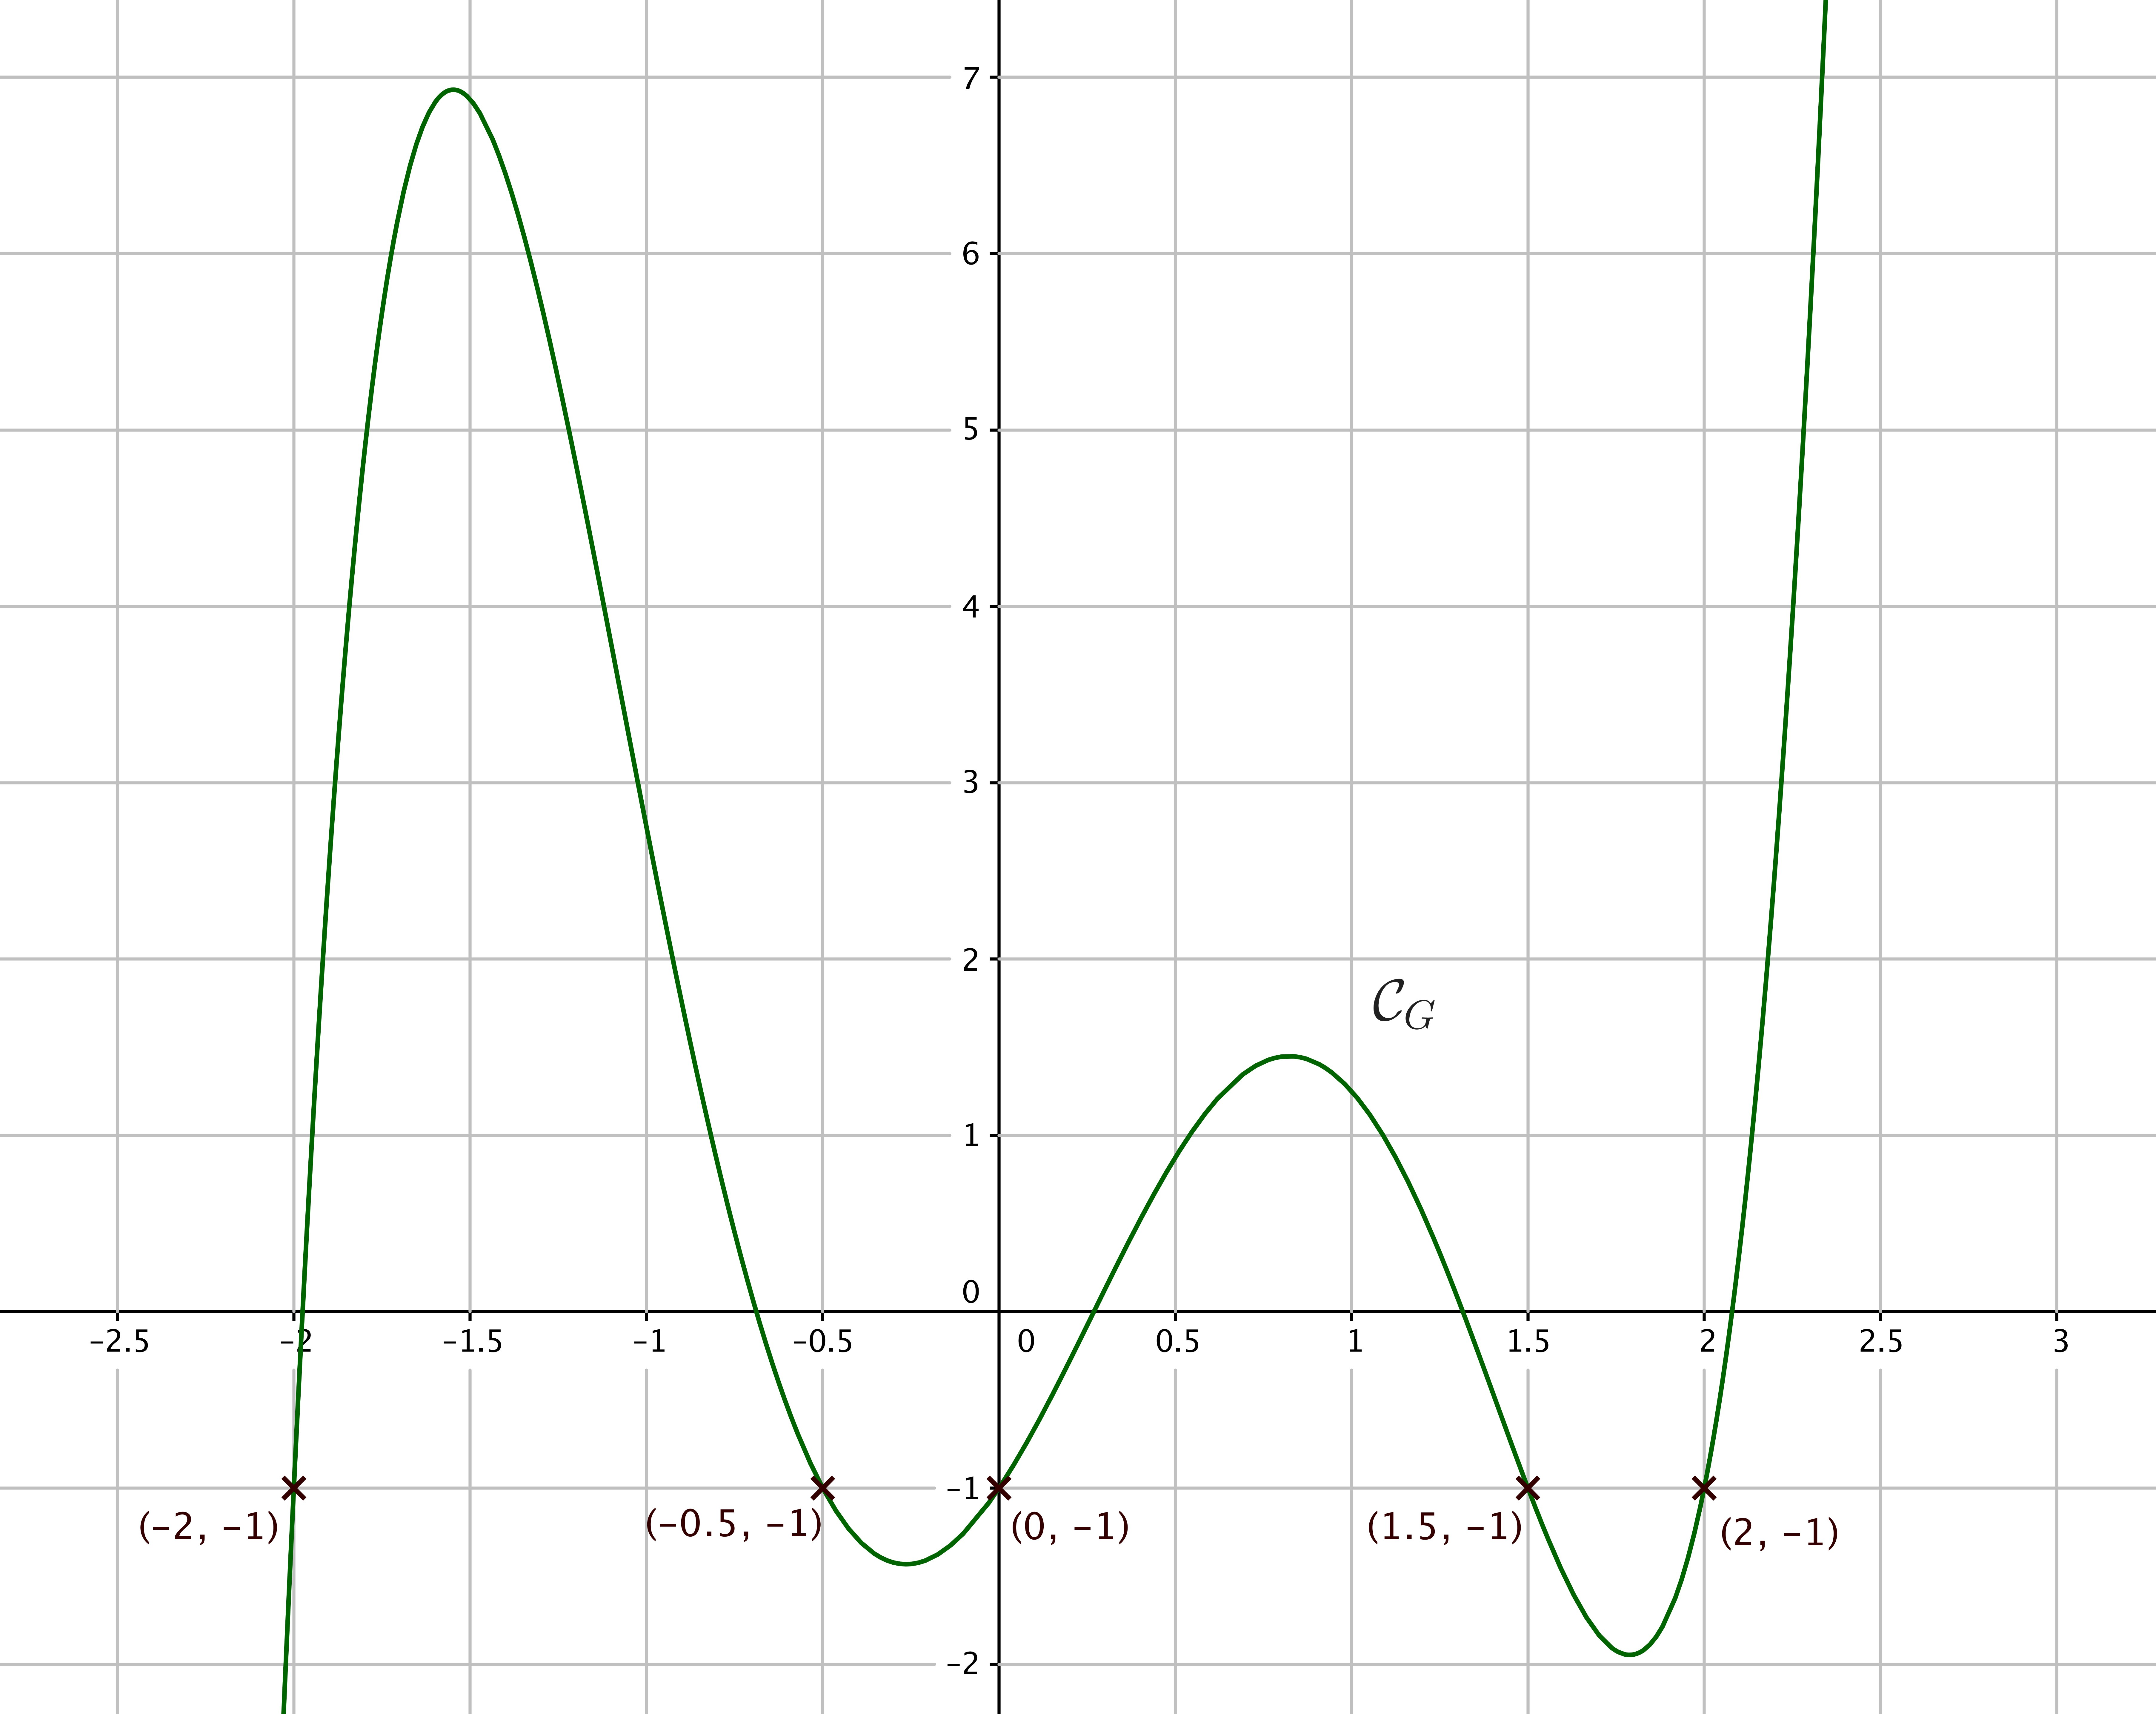
\includegraphics[scale=0.04]{Exo_1.jpg}
	%\label{fig_5}\end{figure*}	
	\end{minipage}\hfil	
	\begin{minipage}[t]{0.45\linewidth}
	$$\shorthandoff{:}\begin{tikzpicture}[scale=1]
	\clip (-3.1,-3.1) rectangle (3.1,3.1);
	\draw[step=0.5,dotted] (-3,-3) grid (3,3);
	\draw [->, line width = 1pt, >=latex'](-3,0) -- (3,0);
	\draw [->, line width = 1pt, >=latex'](0,-3) -- (0,3);
	\draw (0,1) node{$+$} node[above left]{$J$};
	\draw (1,0) node{$+$} node[below left]{$I$};
	\draw (0,0) node{$+$} node[below left]{$O$};
	\draw[domain=-3:3,samples=100,color=blue] plot ({\x},{0.411*\x*(\x+2.5)*(\x-2.5)});
	\draw (2.32,2.7) node[right]{$\mathcal{C}_G$};
	\end{tikzpicture}\shorthandon{:}$$	
	\end{minipage}
	\end{minipage}	
\end{exer}
\newpage

\subsubsection{Signe d'une fonction sur un intervalle et lecture graphique, tableau de signes:}

\noindent\fcolorbox{vert}{white}{\begin{minipage}{1\linewidth}\begin{minipage}{0.97\linewidth}\begin{defi}
		Soient $f$ une fonction définie sur $\R$ et $I$ un intervalle réel.\\[-0.5cm]
		\begin{itemize}
		\item La fonction $f$ est $\dots\dots\dots\dots\dots$ sur $I$ si .\dotfill\\
		\item La fonction $f$ est $\dots\dots\dots\dots\dots$ sur $I$ si .\dotfill\\
		\end{itemize} 
			
		\end{defi}
	\end{minipage}\end{minipage}\hfill\\}\hfill\\

\begin{ex}\hfill\\\begin{minipage}{1\linewidth}
		\begin{minipage}[c]{0.4\linewidth}
		\shorthandoff{:}\begin{tikzpicture}[scale=1]
		\clip (-3.1,-3.1) rectangle (3.1,3.1);
		\draw[step=0.5,dotted] (-3,-3) grid (3,3);
		\draw [->, line width = 1pt, >=latex'](-3,0) -- (3,0);
		\draw [->, line width = 1pt, >=latex'](0,-3) -- (0,3);
		\draw (0,1) node{$+$} node[above left]{$J$};
		\draw (1,0) node{$+$} node[below left]{$I$};
		\draw (0,0) node{$+$} node[below left]{$O$};
		\draw[domain=-3:3,samples=100,color=blue] plot ({\x},{0.411*\x*(\x+2.5)*(\x-2.5)});
		\draw (2.42,2.7) node[right]{$\mathcal{C}_f$};
		\end{tikzpicture}\shorthandon{:}		
		\end{minipage}
		\hfil
		\begin{minipage}[c]{0.49\linewidth}
			.\dotfill \\
			\\
			.\dotfill \\
			\\
			.\dotfill \\
			\\
			.\dotfill \\
			\\
			.\dotfill \\
			\\
		\end{minipage}
\end{minipage}\end{ex} 
\begin{exer}
	Par lecture graphique donner le signe de la fonction $g$.\\\hfill\\
	\begin{minipage}{1\linewidth}
		\begin{minipage}[c]{0.49\linewidth}
			
			.\dotfill \\
			\\
			.\dotfill \\
			\\
			.\dotfill \\
			\\
			.\dotfill \\
			\\

		\end{minipage}\hfill
		\begin{minipage}[c]{0.4\linewidth}
			\raggedleft
			\shorthandoff{:}\begin{tikzpicture}[scale=1]
			\clip (-3.1,-3.1) rectangle (3.1,3.1);
			\draw[step=0.5,dotted] (-3,-3) grid (3,3);
			\draw [->, line width = 1pt, >=latex'](-3,0) -- (3,0);
			\draw [->, line width = 1pt, >=latex'](0,-3) -- (0,3);
			\draw (0,1) node{$+$} node[above left]{$J$};
			\draw (1,0) node{$+$} node[below left]{$I$};
			\draw (0,0) node{$+$} node[below left]{$O$};
			\draw[domain=-3:3,samples=100,color=blue] plot ({\x},{0.25*(\x+1)*(\x+2.5)*(\x-1.5)*(\x-2.5)});
			\draw (2,2.7) node[right]{$\mathcal{C}_g$};
			\end{tikzpicture}\shorthandon{:}		
		\end{minipage}	
	\end{minipage}
\end{exer}

\begin{exer}
	Par lecture graphique donner le signe de la fonction $h$.\\\hfill\\
	\begin{minipage}{1\linewidth}
		\begin{minipage}[c]{0.4\linewidth}
			\shorthandoff{:}\begin{tikzpicture}[scale=1]
			\clip (-3.1,-3.1) rectangle (3.1,3.1);
			\draw[step=0.5,dotted] (-3,-3) grid (3,3);
			\draw [->, line width = 1pt, >=latex'](-3,0) -- (3,0);
			\draw [->, line width = 1pt, >=latex'](0,-3) -- (0,3);
			\draw (0,1) node{$+$} node[above left]{$J$};
			\draw (1,0) node{$+$} node[below left]{$I$};
			\draw (0,0) node{$+$} node[below left]{$O$};
			\draw[domain=-3:3,samples=100,color=blue] plot ({\x},{2.5*cos(pi*\x r)});
			\draw (2,2.7) node[left]{$\mathcal{C}_h$};
			\end{tikzpicture}\shorthandon{:}	
		\end{minipage}
		\hfil
		\begin{minipage}[c]{0.49\linewidth}
			
			.\dotfill \\
			\\
			.\dotfill \\
			\\
			.\dotfill \\
			\\
			.\dotfill \\
			\\

		\end{minipage}
	\end{minipage}
\end{exer}

\newpage

\subsubsection{Résolution d’équations et d’inéquations:}

\fcolorbox{blue}{white}{
	\begin{minipage}[t]{0.95\linewidth}
		\hfill\\
		\noindent\textbf{\underline{Résoudre avec un graphique l'équation $f(x) = k$:}}\\
		\begin{minipage}[c]{0.45\linewidth}
			\begin{enumerate}[I/]
				\item Trouver le nombre $k$ sur l'axe des ordonnées.
				\item Se déplacer horizontalement en restant à la même hauteur pour trouver si il existe un ou des points de $\mathcal{C}_f$. 
				\item Partir des points de $\mathcal{C}_f$ trouvés puis monter ou bien descendre jusqu'à toucher l'axe des abscisses.
				\item Lire les valeurs $x_1$ , $x_2$ et $x_3$ qui sont solutions de l'équation de $f(x) = k$. 
			\end{enumerate}	
		\end{minipage}
	\hfill
		\begin{minipage}[c]{0.4\linewidth}
			\shorthandoff{:}\begin{tikzpicture}[scale=1]
			\clip (-3.1,-3.1) rectangle (3.1,3.1);
			\draw[step=0.5,dotted] (-3,-3) grid (3,3);
			\draw [->, line width = 1pt, >=latex'](-3,0) -- (3,0);
			\draw [->, line width = 1pt, >=latex'](0,-3) -- (0,3);
			\draw (0,1) node{$+$} node[below left]{$J$};
			\draw (1,0) node{$+$} node[below left]{$I$};
			\draw (0,0) node{$+$} node[below left]{$O$};
			\draw[domain=-3:3,samples=100,color=blue] plot ({\x},{0.25*(\x+2.5)*(\x-1.5)*(\x-2.5)-1});
			\draw [line width = 1.7pt, color=brown, dotted] (-3, -1) -- (3,-1);
			\draw (0,-1) node[above right]{$k$};
			\draw [line width = 1.7pt, color=brown, dotted] (-2.5,0) -- (-2.5,-1);
			\draw [line width = 1.7pt, color=brown, dotted] (1.5,0) -- (1.5,-1);
			\draw [line width = 1.7pt, color=brown, dotted] (2.5,0) -- (2.5,-1);
			\draw (-2.5,0) node[above]{$x_1$};
			\draw (1.5,0) node[above]{$x_2$};
			\draw (2.5,0) node[above]{$x_3$};
			\draw (-2.5,-1) node {$\times$};
			\draw (1.5,-1) node {$\times$};
			\draw (2.5,-1) node {$\times$};
			\draw (-1.5,2.2) node[above right]{$\mathcal{C}_f$};
			\end{tikzpicture}\shorthandon{:}		
		\end{minipage}
		\hfill\\ \hfill\\	
\end{minipage}}


\bigskip\bigskip


\fcolorbox{blue}{white}{
	\begin{minipage}[t]{0.95\linewidth}
		\hfill\\
		\noindent\textbf{\underline{Résoudre avec un graphique l'inéquation $f(x) \leq k$:}}\\
		\begin{minipage}[c]{0.45\linewidth}
			\begin{enumerate}[I/]
				\item Trouver le nombre $k$ sur l'axe des ordonnées.
				\item Se déplacer horizontalement en restant à la même hauteur pour trouver si il existe un ou des points de $\mathcal{C}_f$. 
				\item Colorier la partie de $\mathcal{C}_f$ qui est en dessous de la droite d'équation $y=k$.
				\item Lire les valeurs $x_1$ et $x_2$  et donner la réponse sous forme d'intervalle. 
			\end{enumerate}	
		\end{minipage}
		\hfill
		\begin{minipage}[c]{0.4\linewidth}
			\shorthandoff{:}\begin{tikzpicture}[scale=1]
			\clip (-3.1,-3.1) rectangle (3.1,3.1);
			\draw[step=0.5,dotted] (-3,-3) grid (3,3);
			\draw [->, line width = 1pt, >=latex'](-3,0) -- (3,0);
			\draw [->, line width = 1pt, >=latex'](0,-3) -- (0,3);
			\draw (0,1) node{$+$} node[below left]{$J$};
			\draw (1,0) node{$+$} node[below left]{$I$};
			\draw (0,0) node{$+$} node[below left]{$O$};
			\draw[domain=-3:3,samples=100,color=blue] plot ({\x},{0.25*(\x+2.5)*(\x-1.5)-1});
			\draw[domain=-2.5:1.5,line width = 1.7pt,samples=100] plot ({\x},{0.25*(\x+2.5)*(\x-1.5)-1});
			\draw [line width = 1.7pt, color=brown, dotted] (-3, -1) -- (3,-1);
			\draw (0,-1) node[above right]{$k$};
			\draw [line width = 1.7pt, color=brown, dotted] (-2.5,0) -- (-2.5,-1);
			\draw [line width = 1.7pt, color=brown, dotted] (1.5,0) -- (1.5,-1);
			\draw [line width = 1.7pt, color=brown, dotted] (2.5,0) -- (2.5,-1);
			\draw (-2.5,0) node[above]{$x_1$};
			\draw (1.5,0) node[above]{$x_2$};
			\draw (-2.5,-1) node {$\times$};
			\draw (1.5,-1) node {$\times$};
			\draw (3,1) node[above left]{$\mathcal{C}_f$};
			\end{tikzpicture}\shorthandon{:}		
		\end{minipage}
		\hfill\\ \hfill\\	
\end{minipage}}

\begin{ex}\hfill\\\begin{minipage}{1\linewidth}
		\begin{minipage}[c]{0.4\linewidth}
			\shorthandoff{:}\begin{tikzpicture}[scale=1]
			\clip (-3.1,-2.1) rectangle (3.1,3.1);
			\draw[step=0.5,dotted] (-3,-3) grid (3,3);
			\draw [->, line width = 1pt, >=latex'](-3,0) -- (3,0);
			\draw [->, line width = 1pt, >=latex'](0,-3) -- (0,3);
			\draw (0,1) node{$+$} node[below left]{$J$};
			\draw (1,0) node{$+$} node[below left]{$I$};
			\draw (0,0) node{$+$} node[below left]{$O$};
			\draw[domain=-3:3,samples=100,color=blue] plot ({\x},{0.2*\x*(\x+2.5)*(\x-2.5)+1.5});
			\draw (2,2.7) node[right]{$\mathcal{C}_f$};
			\end{tikzpicture}\shorthandon{:}		
		\end{minipage}
		\hfil
		\begin{minipage}[c]{0.49\linewidth}
			\begin{enumerate}
				\item Résoudre graphiquement l'équation $f(x) = 1.5$:\\[0.5cm]
				.\dotfill \\
				\\
				.\dotfill \\
				\item Résoudre graphiquement l'inéquation $f(x) \leq 1.5$:\\[0.5cm]
				.\dotfill \\
				\\
				.\dotfill \\
			\end{enumerate}

		\end{minipage}
\end{minipage}\end{ex} 

\newpage
\begin{exer}
	\hfill\\\hfill\\
	\begin{minipage}{1\linewidth}
		\begin{minipage}[c]{0.49\linewidth}
		\item Résoudre graphiquement l'équation $g(x) = 0.5$:\\[0.5cm]
		.\dotfill \\
		\\
		.\dotfill \\
		\item Résoudre graphiquement l'inéquation $g(x) < 0.5$:\\[0.5cm]
		.\dotfill \\
		\\
		.\dotfill \\
			
		\end{minipage}\hfill
		\begin{minipage}[c]{0.4\linewidth}
			\raggedleft
			\shorthandoff{:}\begin{tikzpicture}[scale=1]
			\clip (-3.1,-3.1) rectangle (3.1,3.1);
			\draw[step=0.5,dotted] (-3,-3) grid (3,3);
			\draw [->, line width = 1pt, >=latex'](-3,0) -- (3,0);
			\draw [->, line width = 1pt, >=latex'](0,-3) -- (0,3);
			\draw (0,1) node{$+$} node[above left]{$J$};
			\draw (1,0) node{$+$} node[below left]{$I$};
			\draw (0,0) node{$+$} node[below left]{$O$};
			\draw[domain=-3:3,samples=100,color=blue] plot ({\x},{-0.25*(\x+1)*(\x+2.5)*(\x-1.5)*(\x-2.5)+0.5});
			\draw (2,1.35) node[above right]{$\mathcal{C}_g$};
			\end{tikzpicture}\shorthandon{:}		
		\end{minipage}	
	\end{minipage}
\end{exer}

\begin{exer}
	\hfill\\\hfill\\
	\begin{minipage}{1\linewidth}
		\begin{minipage}[c]{0.4\linewidth}
			\shorthandoff{:}\begin{tikzpicture}[scale=1]
			\clip (-3.1,-1.5) rectangle (3.1,3.1);
			\draw[step=0.5,dotted] (-3,-3) grid (3,3);
			\draw [->, line width = 1pt, >=latex'](-3,0) -- (3,0);
			\draw [->, line width = 1pt, >=latex'](0,-3) -- (0,3);
			\draw (0,1) node{$+$} node[above left]{$J$};
			\draw (1,0) node{$+$} node[below left]{$I$};
			\draw (0,0) node{$+$} node[below right]{$O$};
			\draw[domain=-3:3,samples=100,color=blue] plot ({\x},{1.5*sin(pi*\x r)+1});
			\draw (2.6,2.7) node[left]{$\mathcal{C}_h$};
			\end{tikzpicture}\shorthandon{:}	
		\end{minipage}
		\hfil
		\begin{minipage}[c]{0.49\linewidth}
		\item Résoudre graphiquement l'équation $h(x) = 1$:\\[0.5cm]
		.\dotfill \\
		\\
		.\dotfill \\
		\item Résoudre graphiquement l'inéquation $h(x) \geq 1$:\\[0.5cm]
		.\dotfill \\
		\\
		.\dotfill \\
			
		\end{minipage}
	\end{minipage}
\end{exer}
\section{Variations et extremums:}
\subsection{Variation d'une fonction sur un intervalle:}

\noindent\fcolorbox{vert}{white}{\begin{minipage}{1\linewidth}\begin{defi}
			Soient $f$ une fonction définie sur $\R$ et $I$ un intervalle réel.\\[-0.5cm]
			\begin{itemize}
				\item La fonction $f$ est $\dots\dots\dots\dots\dots$ sur $I$ si .\dotfill\\
				.\dotfill\\.\dotfill\\[-0.5cm]
				\item La fonction $f$ est $\dots\dots\dots\dots\dots$ sur $I$ si .\dotfill\\
				.\dotfill\\.\dotfill\\
			\end{itemize}\end{defi}\end{minipage}\hfill\\}\hfill\\

\begin{rmq}\hfil\\[-0.5cm]
	\begin{enumerate}[$\square$]
		\item Un fonction est croissante sur un intervalle $I$ si elle garde le même ordre au départ qu'à l'arrivée.  
		\item Un fonction est décroissante sur un intervalle $I$ si elle change l'ordre entre le départ et l'arrivée.
	\end{enumerate}
\end{rmq}
\newpage
\begin{ex}\hfill\\[0.5cm]\begin{minipage}{1\linewidth}
		\begin{minipage}[c]{0.4\linewidth}
			\shorthandoff{:}\begin{tikzpicture}[scale=1]
			\clip (-2.4,-3.6) rectangle (3.4,3.6);
			\draw[step=0.5,dotted] (-3.5,-3.5) grid (3.5,3.5);
			\draw [->, line width = 1pt, >=latex'](-3.5,0) -- (3.4,0);
			\draw [->, line width = 1pt, >=latex'](0,-3.5) -- (0,3.5);
			\draw (0,1) node{$+$} node[above left]{$J$};
			\draw (1,0) node{$+$} node[below left]{$I$};
			\draw (0,0) node{$+$} node[below left]{$O$};
			\draw[domain=-3.6:3.6,samples=100,color=blue] plot ({\x},{(\x+1)*(\x-2)+0.25});
			\draw (2.1,2.7) node[right]{$\mathcal{C}_f$};
			\end{tikzpicture}\shorthandon{:}		
		\end{minipage}
		\hfil
		\begin{minipage}[c]{0.49\linewidth}
			.\dotfill \\
			\\
			.\dotfill \\
			\\
			.\dotfill \\
			\\
			.\dotfill \\
			\\
			.\dotfill \\
			\\
			.\dotfill \\
			\\
		\end{minipage}
\end{minipage}\end{ex} 

\begin{ex}\hfill\\[0.5cm]\begin{minipage}{1\linewidth}
		\begin{minipage}[c]{0.49\linewidth}
			\hfill\\
			.\dotfill \\
			\\
			.\dotfill \\
			\\
			.\dotfill \\
			\\
			.\dotfill \\
			\\
			.\dotfill \\
			\\

		\end{minipage}\hfill
	\begin{minipage}[c]{0.4\linewidth}
		\shorthandoff{:}\begin{tikzpicture}[scale=1]
		\clip (-3.4,-3.6) rectangle (3.4,3.6);
		\draw[step=0.5,dotted] (-3.5,-3.5) grid (3.5,3.5);
		\draw [->, line width = 1pt, >=latex'](-3.5,0) -- (3.4,0);
		\draw [->, line width = 1pt, >=latex'](0,-3.5) -- (0,3.5);
		\draw (0,1) node{$+$} node[above left]{$J$};
		\draw (1,0) node{$+$} node[below left]{$I$};
		\draw (0,0) node{$+$} node[below left]{$O$};
		\draw[domain=-3.6:3.6,samples=100,color=blue] plot ({\x},{1/3*\x^3- (1.5)^2*\x+0.25});
		\draw (2.42,2.7) node[right]{$\mathcal{C}_g$};
		\end{tikzpicture}\shorthandon{:}		
	\end{minipage}
\end{minipage}\end{ex}
\begin{exer}\hfill\\[0.5cm]\begin{minipage}{1\linewidth}
		\begin{minipage}[c]{0.4\linewidth}
			\shorthandoff{:}\begin{tikzpicture}[scale=1]
			\clip (-3.1,-2) rectangle (3.1,3.1);
			\draw[step=0.5,dotted] (-3,-3) grid (3,3);
			\draw [->, line width = 1pt, >=latex'](-3,0) -- (3,0);
			\draw [->, line width = 1pt, >=latex'](0,-3) -- (0,3);
			\draw (0,1) node{$+$} node[above left]{$J$};
			\draw (1,0) node{$+$} node[below left]{$I$};
			\draw (0,0) node{$+$} node[below right]{$O$};
			\draw[domain=-3:3,samples=100,color=blue] plot ({\x},{1.5*sin(pi/3*\x r)+0.5});
			\draw (2,2.7) node[left]{$\mathcal{C}_h$};
			\end{tikzpicture}\shorthandon{:}		
		\end{minipage}
		\hfil
		\begin{minipage}[c]{0.49\linewidth}
			À l'aide de la courbe représentative de la fonction $h$ donner le tableau de variation de la fonction $h$. 
			\\[0.5cm]
			.\dotfill \\
			\\
			.\dotfill \\
			\\
			.\dotfill \\
			\\
			.\dotfill \\
			\\

		\end{minipage}
\end{minipage}\end{exer} 

\noindent \textbf{\textcolor{purple}{$
\includegraphics[scale=0.05]{logo-td.png}$ \ Exercices 20 ,22 et 23 p.185}} \\



\newpage
\subsection{Extremums d'une fonction sur un intervalle:}

\noindent\fcolorbox{vert}{white}{\begin{minipage}{1\linewidth}\begin{defi}
			Soient $f$ une fonction définie sur $\R$, $I$ un intervalle réel et $x_1,x_2\in I$.\\[-0.5cm]
			\begin{itemize}
				\item La fonction $f$ admet un $\dots\dots\dots\dots\dots\dots\dots\dots\dots\dots\dots$ en $x_1$ sur $I$ si  .\dotfill\\
				.\dotfill\\[-0.5cm]
				\item La fonction $f$ admet un $\dots\dots\dots\dots\dots\dots\dots\dots\dots\dots\dots$ en $x_2$ sur $I$ si .\dotfill\\
				.\dotfill\\
	\end{itemize}\end{defi}\end{minipage}\hfill\\}\hfill\\

\begin{ex}\hfill\\[0.5cm]\begin{minipage}{1\linewidth}
		\begin{minipage}[c]{0.4\linewidth}
			\shorthandoff{:}\begin{tikzpicture}[scale=1]
			\clip (-2.4,-3.6) rectangle (3.4,3.6);
			\draw[step=0.5,dotted] (-3.5,-3.5) grid (3.5,3.5);
			\draw [->, line width = 1pt, >=latex'](-3.5,0) -- (3.4,0);
			\draw [->, line width = 1pt, >=latex'](0,-3.5) -- (0,3.5);
			\draw (0,1) node{$+$} node[above left]{$J$};
			\draw (1,0) node{$+$} node[below left]{$I$};
			\draw (0,0) node{$+$} node[below left]{$O$};
			\draw[domain=-3.6:3.6,samples=100,color=blue] plot ({\x},{(\x+1)*(\x-2)+0.25});
			\draw (2.1,2.7) node[right]{$\mathcal{C}_f$};
			\end{tikzpicture}\shorthandon{:}		
		\end{minipage}
		\hfil
		\begin{minipage}[c]{0.49\linewidth}
			.\dotfill \\
			\\
			.\dotfill \\
			\\
			.\dotfill \\
			\\
			.\dotfill \\
			\\
			.\dotfill \\
			\\
			.\dotfill \\
			\\
		\end{minipage}
\end{minipage}\end{ex} 

\begin{ex}\hfill\\[0.5cm]\begin{minipage}{1\linewidth}
		\begin{minipage}[c]{0.49\linewidth}
			\hfill\\
			.\dotfill \\
			\\
			.\dotfill \\
			\\
			.\dotfill \\
			\\
			.\dotfill \\
			\\
			.\dotfill \\
			\\
			
		\end{minipage}\hfill
		\begin{minipage}[c]{0.4\linewidth}
			\shorthandoff{:}\begin{tikzpicture}[scale=1]
			\clip (-3.4,-3.6) rectangle (3.4,3.6);
			\draw[step=0.5,dotted] (-3.5,-3.5) grid (3.5,3.5);
			\draw [->, line width = 1pt, >=latex'](-3.5,0) -- (3.4,0);
			\draw [->, line width = 1pt, >=latex'](0,-3.5) -- (0,3.5);
			\draw (0,1) node{$+$} node[above left]{$J$};
			\draw (1,0) node{$+$} node[below left]{$I$};
			\draw (0,0) node{$+$} node[below left]{$O$};
			\draw[domain=-3.6:3.6,samples=100,color=blue] plot ({\x},{1/3*\x^3- (1.5)^2*\x+0.25});
			\draw (2.42,2.7) node[right]{$\mathcal{C}_g$};
			\end{tikzpicture}\shorthandon{:}		
		\end{minipage}
\end{minipage}\end{ex}

\noindent \textbf{\textcolor{purple}{$
\includegraphics[scale=0.05]{logo-td.png}$ \ Exercice 40 p.188 - Exercice 33 et 36 p.187 }} \\


\end{document}



